\documentclass[pdf,aspectratio=169]{beamer}
\usepackage[]{hyperref,graphicx,siunitx,booktabs,lmodern}
\usepackage{physics}
\usepackage{em-commands}
\mode<presentation>{\usetheme{EM}}

%Question Numbering
\newcounter{questionnumber}
\newcommand{\qnum}{%
	\stepcounter{questionnumber}%
	Q\arabic{questionnumber}
}
\resetcounteronoverlays{questionnumber}

\graphicspath{ {../Images/} }

\sisetup{per-mode=symbol}

%preamble
\title{Simple Induction My Dear Watson}
\date{December 5, 2018}
\author{Jed Rembold}

\begin{document}
\renewcommand{\theenumi}{\Alph{enumi}}

\begin{frame}{Announcements}
	\begin{itemize}
		\item Happy Birthday Griffiths (and Ricky!)
		\item Homework
			\begin{itemize}
				\item Homework 12 due tonight!
			\end{itemize}
		\item Final
			\begin{itemize}
				\item Coming at you Friday!
				\item Due the 14th at 5pm
				\item Probably looking at around 5-6 problems
				\item Chapters 6 and 7 will be weighted a bit heavier, but it is comprehensive
				\item Come the moment I send it out, my solutions sets will be locked down (figuratively)
				\item Total learning objectives posted on Campuswire
			\end{itemize}
		\item On Friday
			\begin{itemize}
				\item Talking Maxwell's Laws
				\item Class picture
				\item And my evaluations!
					\begin{itemize}
						\item I'm particularly interested how you felt about the way lectures were done this semester
					\end{itemize}
			\end{itemize}
		\item Read rest of Ch 7 for Friday
	\end{itemize}
\end{frame}

\begin{frame}{\qnum}
	\begin{columns}
		\column{0.5\textwidth}
		The current in an infinite solenoid with uniform magnetic field is increasing such that $B = B_0 + kt$. If you calculate the potential between points A and B along the two different paths shown, do you get the same answer?

		\begin{enumerate}
			\item \alert<2>{Yes}
			\item No
			\item Can't tell with current info
			\item Only at certain times
		\end{enumerate}
		
		\column{0.5\textwidth}
		\begin{center}
			\begin{tikzpicture}[use quick Hobby shortcut]
				\node[font=\Large,above] at (0,-3) {Top View};
				\draw[very thick, fill=Red!70] (0,0) circle (2);
				\node[label=$\mf$] at (0,0) {$\odot$};
				\node[point,label={-90:A}](A) at (45:2.5) {};
				\node[point,label={270:B}](B) at (180+45:2.5) {};

				\draw[very thick, ->>-=0.1 to .9 by .2] (A) to[quick curve through={(90:4) (135:3) (180:4)}] (B);
				\draw[very thick, ->>-=0.1 to .9 by .2] (A) to[quick curve through={(90:3) (135:2.25) (180:2.5)}] (B);
			\end{tikzpicture}
		\end{center}
	\end{columns}
\end{frame}

\begin{frame}{\qnum}
	\begin{columns}
		\column{0.5\textwidth}
		If the arrows represent an $\ef$, what can you say about the rate of change in the magnetic flux (perpendicular to the page) through the dashed region? Take positive flux to be out of the page.
		\begin{enumerate}
			\item $\displaystyle \dv{B}{t} > 0$
			\item $\displaystyle \dv{B}{t} < 0$
			\item \alert<2>{$\displaystyle \dv{B}{t} = 0$}
			\item Impossible to say
		\end{enumerate}
		
		\column{0.5\textwidth}
		\begin{center}
			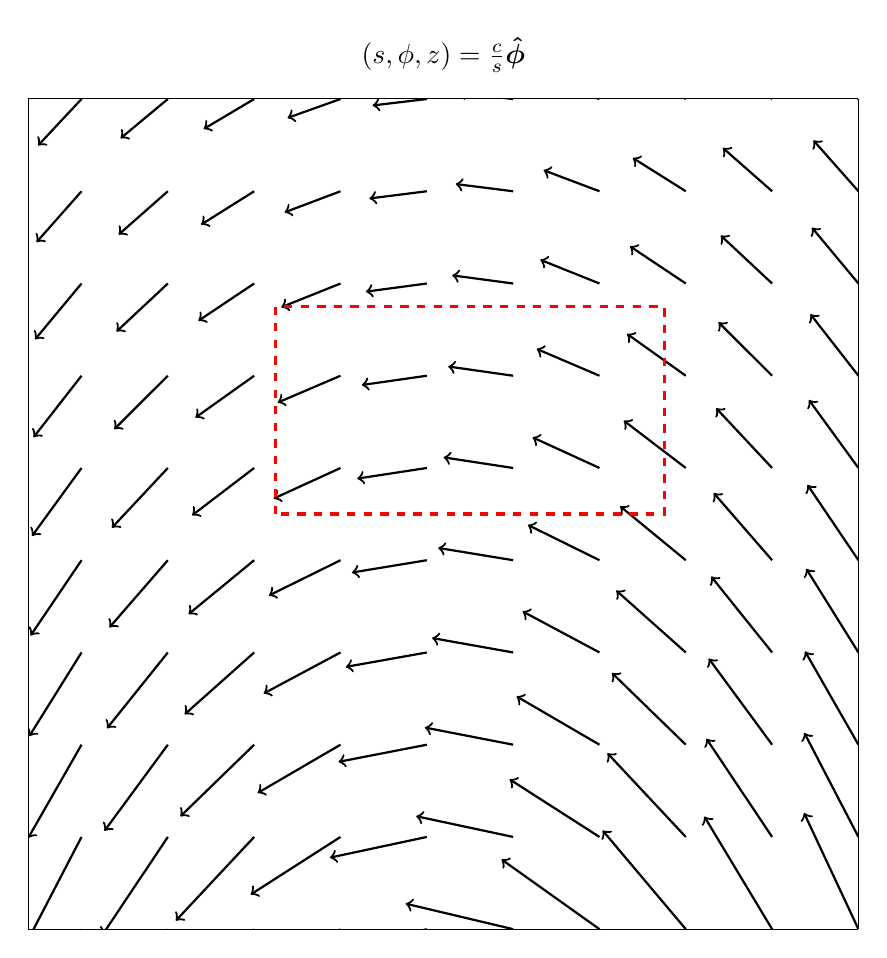
\begin{tikzpicture}
				\begin{axis}[
					domain = -1:1,
					y domain = 1:2,
					title = {$\ef(s,\phi,z) = \frac{c}{s}\vu*\phi$},
					view = {0}{90},
					samples = 10,
					ticks = none,
					width=\textwidth,
					height=\textwidth,
					ymin=1, ymax=2,
					]
					\addplot3[thick, quiver={u={-y/(x^2+y^2)}, v={x/(x^2+y^2)}, scale arrows=0.28}, ->] (x,y,0);
					\draw[very thick, red, dashed] (axis cs: -.5,1.5) rectangle (axis cs: .5,1.75);
				\end{axis}
			\end{tikzpicture}
		\end{center}
	\end{columns}
\end{frame}

\begin{frame}{\qnum}
	\begin{columns}
		\column{0.5\textwidth}
		\begin{center}
			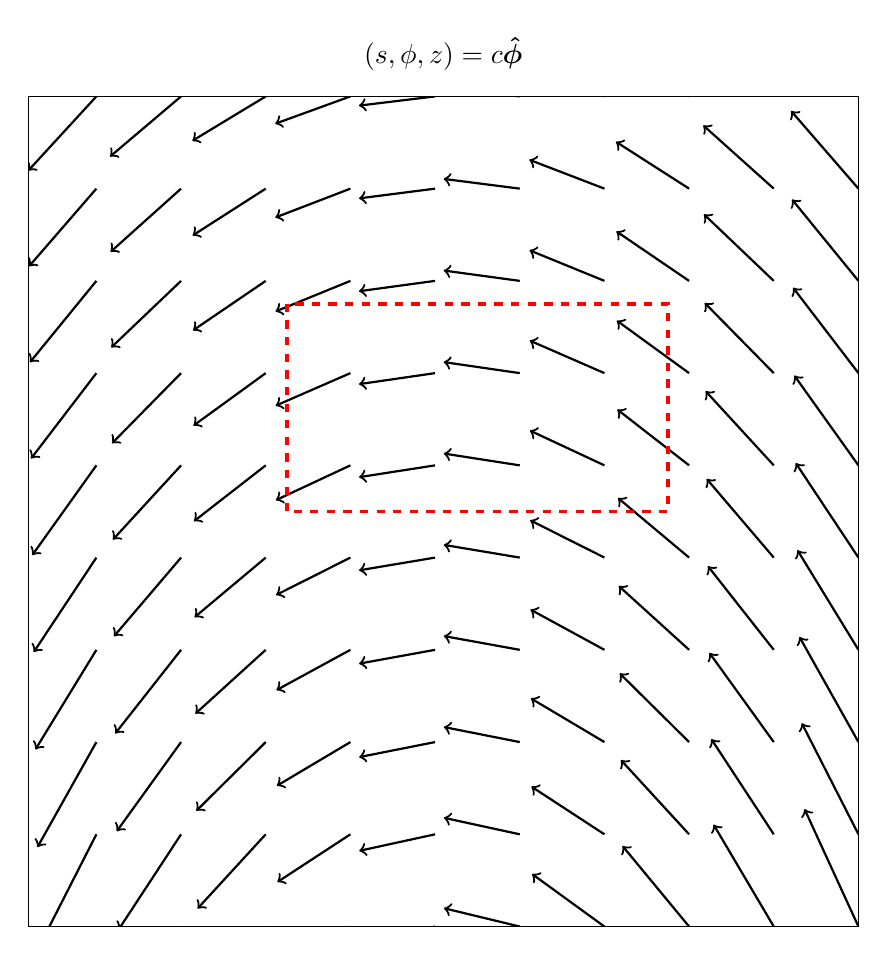
\begin{tikzpicture}
				\begin{axis}[
					domain = -1:1,
					y domain = 1:2,
					title = {$\ef(s,\phi,z) = c\vu*\phi$},
					view = {0}{90},
					samples = 10,
					ticks = none,
					width=\textwidth,
					height=\textwidth,
					ymin=1, ymax=2,
					]
					\addplot3[thick, quiver={u={-y/(x^2+y^2)^.5}, v={x/(x^2+y^2)^.5}, scale arrows=0.20}, ->] (x,y,0);
					\draw[very thick, red, dashed] (axis cs: -.5,1.5) rectangle (axis cs: .5,1.75);
				\end{axis}
			\end{tikzpicture}
		\end{center}

		\column{0.5\textwidth}
		If the arrows represent an $\ef$, what can you say about the rate of change in the magnetic flux (perpendicular to the page) through the dashed region? Take positive flux to be out of the page.
		\begin{enumerate}
			\item $\displaystyle \dv{B}{t} > 0$
			\item \alert<2>{$\displaystyle \dv{B}{t} < 0$}
			\item $\displaystyle \dv{B}{t} = 0$
			\item Impossible to say
		\end{enumerate}
		\end{columns}
\end{frame}

\begin{frame}{\qnum}
	\begin{columns}
		\column{0.5\textwidth}
		The current $\mcur_1$ in loop 1 is increasing. What is the direction of the induced current in loop 2, which is coaxial with loop 1?
		\begin{enumerate}
			\item Same direction as $\cur_1$
			\item \alert<2>{Opposite direction of $\cur_1$}
			\item There is no induced current
			\item It depends on the distance between the loops
		\end{enumerate}
		
		\column{0.5\textwidth}
		\begin{center}
			\begin{tikzpicture}
				\node[label={right:2}](2) at (2,2) {};
				\node[label={right:1}](1) at (3,0) {};
				\draw[very thick, Red, ->>-=0.1 to .9 by .3, dashed] (1) arc (0:180:3cm and .5cm);
				\draw[very thick, Red, ->>-=0.1 to .9 by .3] (1)++(-6,0) arc (180:360:3cm and .5cm);
				\draw[very thick, dashed] (2) arc (0:180:2cm and .25cm);
				\draw[very thick] (2)++(-4,0) arc (180:360:2cm and .25cm);
				\draw[thick, -latex] (0,0) -- +(0,3);
			\end{tikzpicture}
		\end{center}
		
	\end{columns}
\end{frame}

\begin{frame}{\qnum}
		The current $\mcur_1$ in loop 1 is increasing. What is the direction of the induced current in loop 2, which is coaxial with loop 1?
		\begin{center}
			\begin{tikzpicture}
				\node[label={right:2}](2) at (8,0) {};
				\node[label={right:1}](1) at (3,0) {};
				\draw[very thick, Red, ->>-=0.1 to .9 by .3, dashed] (1) arc (0:180:3cm and .5cm);
				\draw[very thick, Red, ->>-=0.1 to .9 by .3] (1)++(-6,0) arc (180:360:3cm and .5cm);
				\draw[very thick, dashed] (2) arc (0:180:2cm and .25cm);
				\draw[very thick] (2)++(-4,0) arc (180:360:2cm and .25cm);
			\end{tikzpicture}
		\end{center}
		\begin{enumerate}
			\item \alert<2>{Same direction as $\cur_1$}
			\item Opposite direction of $\cur_1$
			\item There is no induced current
			\item It depends on the distance between the loops
		\end{enumerate}
\end{frame}

\begin{frame}{\qnum}
	\begin{columns}
		\column{0.5\textwidth}
		A wire (1) is looped around a very long solenoid (2).
		\begin{align*}
			\Phi_1 &= M_{12}\mcur_2 = \text{ flux through loop 1 due to current in 2} \\
			\Phi_2 &= M_{21}\mcur_1 = \text{ flux through solenoid due to current in 1}
		\end{align*}
		Which $M$ is easier to compute?
		\begin{enumerate}
			\item \alert<2>{$M_{12}$}
			\item $M_{21}$
			\item They are equally difficult to compute
			\item Can't say with this information
		\end{enumerate}
		
		\column{0.5\textwidth}
		\begin{center}
			\begin{tikzpicture}
				\coordinate (1) at (2,-4);
				\coordinate (2) at (-2,-3);

				\draw[ultra thick] (1) .. controls +(45:1) and +(45:1).. (2);

				\pic (s) at (0,0) {cyl=orange/1/6/6};
				\foreach \y in {.5,1,...,5.5}{
					\draw[ultra thick, Teal, ->-=0.5] (s-lb)++(0,\y) .. controls +(180+35:.75) and +(-35:.75) .. +(2,0);
				}
				\draw[ultra thick] (2) .. controls +(225:1) and +(225:1).. (1);

				\node[above=5mm] at (0,0) {2};
				\node[left] at (2) {1};
			\end{tikzpicture}
		\end{center}
	\end{columns}
\end{frame}

%\begin{frame}{\qnum}
	%At the indicated position on the parallel plate capacitor, what can you say about the sign of $\div \vcd$? You can assume that $\mcur\neq 0$.
	%\begin{center}
		%\begin{tikzpicture}
			%\node[block, minimum height=3cm] (l) at (-2,0) {};
			%\node[block, minimum height=3cm, fill=blue!50] (r) at (2,0) {};
			%\draw[very thick, ->-=.5] (r.east) -- +(2,0) node[right] {$\mcur$};
			%\draw[very thick, -<-=.5] (l.west) -- +(-2,0) node[left] {$\mcur$};
			%\draw[very thick,Teal,latex-] (l.east) -- +(45:1) node[right] {Here};
		%\end{tikzpicture}
	%\end{center}
	%\begin{enumerate}
		%\item $\div\vcd < 0$
		%\item $\div\vcd > 0$
		%\item $\div\vcd = 0$
		%\item Can't say from this information
	%\end{enumerate}
%\end{frame}



\end{document}
